\chapter{Preprocessing of the data}
\label{ch:prepro}

Before the analysis steps done in this work can be performed, the raw data taken by the LST-1 has to be processed up until what is called Data Level 1 (DL1).
For this work such preprocessing was done using \texttt{lstchain}, a low-level data processing pipeline for the LST telescopes. 
\texttt{lstchain} is open-source project which still in development on github \cite{lstchain} and is based on \texttt{ctapipe}. 
\texttt{ctapipe} will be the main low-level data processing pipeline for CTA and is itself still getting developed as an open-source project.
This work uses the versions \texttt{v0.5.1} and \texttt{v0.5.2} of \texttt{lstchain} which are both based on version \texttt{v0.7.0} of \texttt{ctapipe} \cite{ctapipe}. 

In the first step the waveforms recorded by each pixel of the camera are smoothed and calibrated according to environmental effects to reduce the influence
of electronic noise in the signal.
After that the waveforms are integrated to obtain the total photon charge and a mean arrival time for the photons is defined for each pixel 
as the rising edge of the waveform.
This results in two 2-dimensional images for each event recorded by the camera, as can be seen in \autoref{fig:eas_images}.
\begin{figure}
    \centering
    \begin{subfigure}{0.49\textwidth}
        \centering
        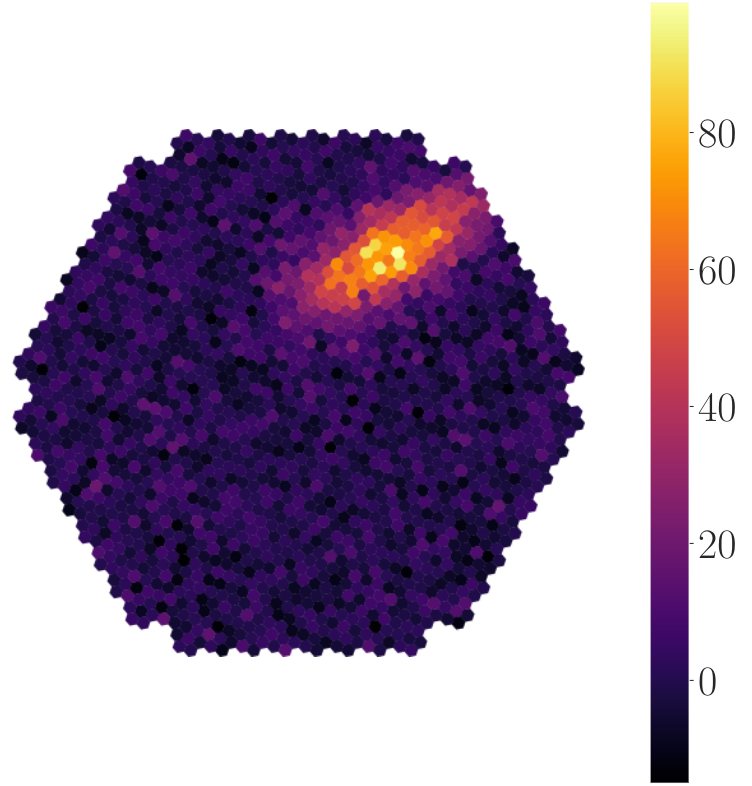
\includegraphics[width=0.8\textwidth]{images/eas_image1.png}
        \caption{Number of photons per pixel.}
        \label{fig:eas_image1}
    \end{subfigure}
    \hfill
    \begin{subfigure}{0.49\textwidth}
        \centering
        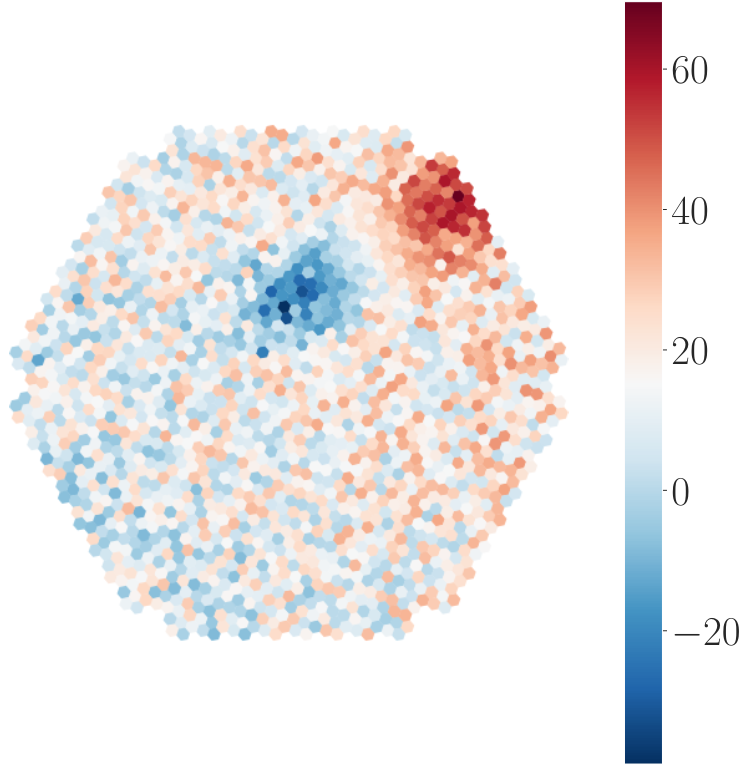
\includegraphics[width=0.8\textwidth]{images/eas_image2.png}
        \caption{Arrival time per pixel relative to the mean arrival time for the whole image.}
        \label{fig:eas_image2}
    \end{subfigure}
    \caption{The integrated photon count in \subref{fig:eas_image1} showes the air shower clearly but a lot of noise is visible in the non-shower pixels.
        The arrival times in \subref{fig:eas_image2} show a clear correlation for the pixels that recorded the air shower \cite{lukas}.
    }
    \label{fig:eas_images}
\end{figure}

In the next step these images are cleaned by discarding pixels that did not record the air shower. 
This is done in multiple using two thresholds for the photon charge of each pixel and one for the number of neighboring pixels.
First all pixels above the higher photon charge threshold with enough neighboring pixels above the lower photon charge threshold get selcted.
After that all pixels above the lower photon charge threshold with enough neighboring pixels above the higher photon charge threshold get selcted as well \cite{lukas}.
For rather soft thresholds the results of this cleaning can be seen in \autoref{fig:eas_images_cleaned}.
\begin{figure}
    \centering
    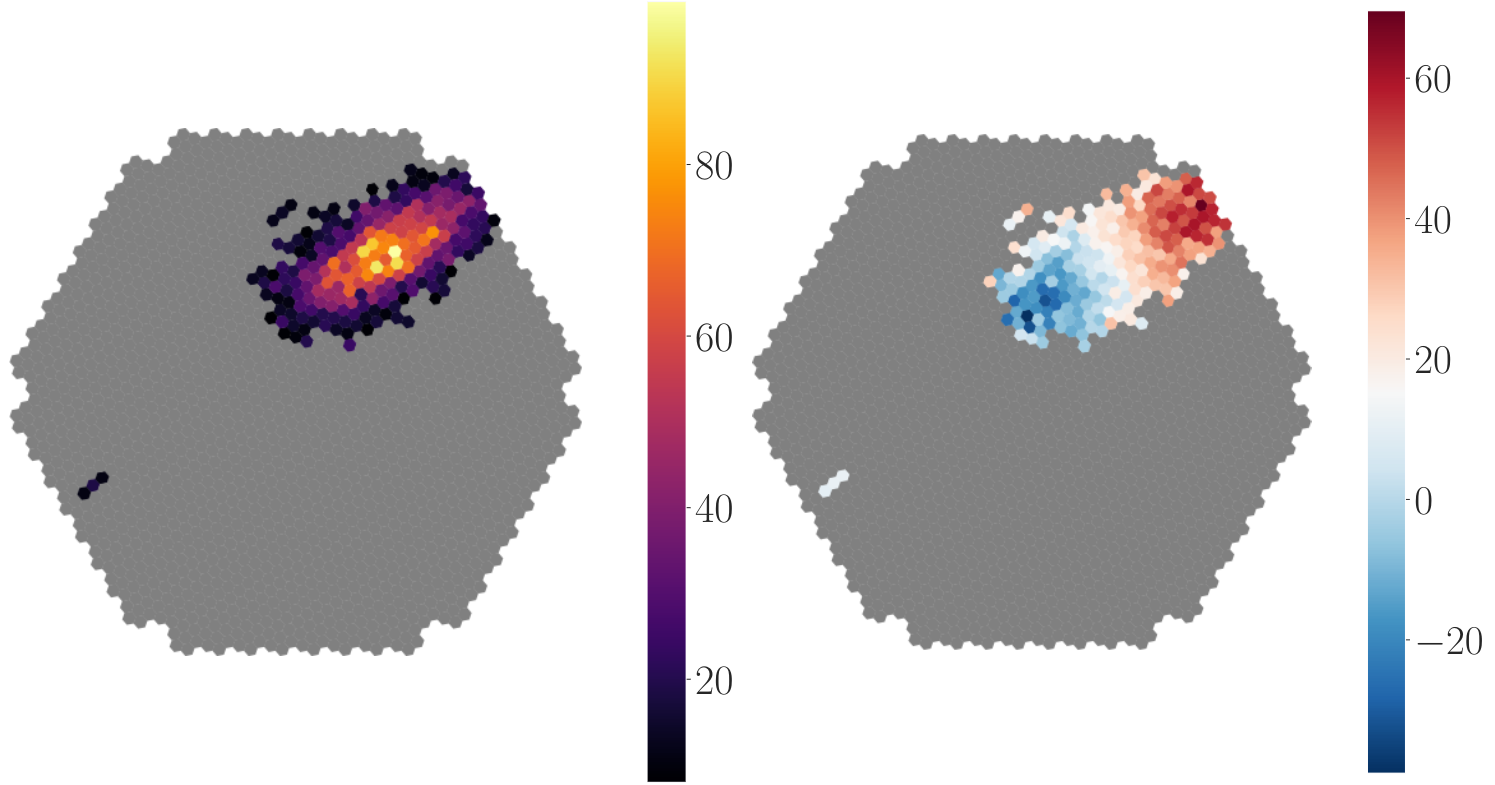
\includegraphics[width=0.8\textwidth]{images/eas_images_cleaned.png}
    \caption{The pixels discarded during the image cleaning are marked as grey. The soft thresholds result in two smaller pixel-islands remaining \cite{lukas}.}
    \label{fig:eas_images_cleaned}
\end{figure}

Based on these cleaned images a multitude of image paramters can be calculated.
The most important ones are the total number of photons in the shower, \texttt{intensity}, and the so called hillas parameters which are illustrated in \autoref{fig:image_parameters}.
the hillas parameters are based on a principal component analysis (PCA) of the photon charge distribution and describe the extension and orientation of the shower.
The parameters \texttt{length} and \texttt{width} correspond with the standart deviations along the principal components of the distribution and are therefore a 
description of the shower extension. 
The orientation on the other hand is described by the angle of the main shower axis relative to the x-axis of the image.
The performance of the algorithms used in this work in regards to reconstructing this angle can be seen in \autoref{fig:delta_comparison}.
\begin{figure}
    \centering
    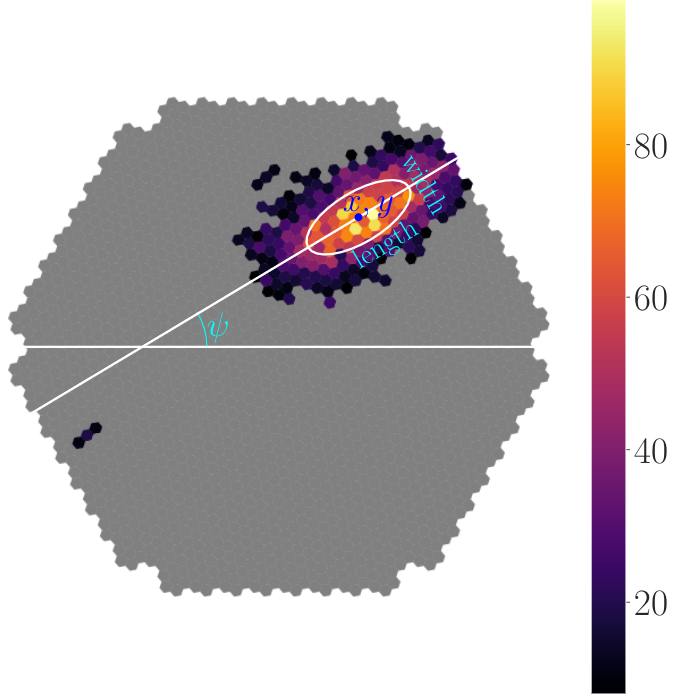
\includegraphics[width=0.5\textwidth]{images/image_parameters.png}
    \caption{The PCA-based hillas-parameters calculated for the cleaned image of the integrated photon count.
        $\Psi$ describes the angle of the main shower axis relative to the x-axis of the image and $x$ and $y$ are the coordinates of the center of gravity of the shower. 
        \texttt{length} and \texttt{width} can be depicted as the semi-major and semi-minor axis of an ellipse \cite{lukas}.
    }
    \label{fig:image_parameters}
\end{figure}

Higher moments of the distribution like \texttt{skewness} and \texttt{kurtosis} are also calculated. 
The center of gravity of the shower image is calculated by weighting the coordinates of each pixel with the photon charge of this pixel.
Additional image featueres include multiple \texttt{leakage} parameters that describe how much of the light was recorded at the edge of the camera and are
therefore an indication of how much light from the shower might have missed the camera.

The image of the arrival times allows for timing paramters to be calculated by fitting a linear function along the main shower axis. 
This yields the parameters \texttt{time\_gradient} and \texttt{intercept} which help to determine the direction of the shower, together with \texttt{skewness} and \texttt{kurtosis}.